\begin{proof}
	Пусть выполнено $A \leqsim B$ и $B \leqsim A$. Это означает, что есть биекции $f \colon A \to B_1$ и $g \colon B \to A_1$, где $A_1 \subset A$ и $B_1 \subset B$.
	
	Так как $f$ и $g$ - отображения, то можно посмотреть на образы $f(A_1) = B_2$ и $g(B_1) = A_2$. При этом верны утверждения:
	\begin{align*}
		&{B \supset B_1 \Ra g(B) \supset g(B_1)}
		\\
		&{A \supset A_1 \Ra f(A) \supset f(A_1)}
	\end{align*}
	То есть $B_1 \supset B_2$ и $A_1 \supset A_2$. Так можно продолжать итеративно и, положив за $A_0 = A$, $B_0 = B$, получить последовательности вложенных множеств:
	\begin{align*}
		&{A_0 \supset A_1 \supset A_2 \supset \ldots}
		\\
		&{B_0 \supset B_1 \supset B_2 \supset \ldots}
	\end{align*}
	При этом имеются равенства:
	\begin{align*}
		&{f(A_k) = B_{k + 1}}
		\\
		&{g(B_k) = A_{k + 1}}
	\end{align*}

	\begin{center}
		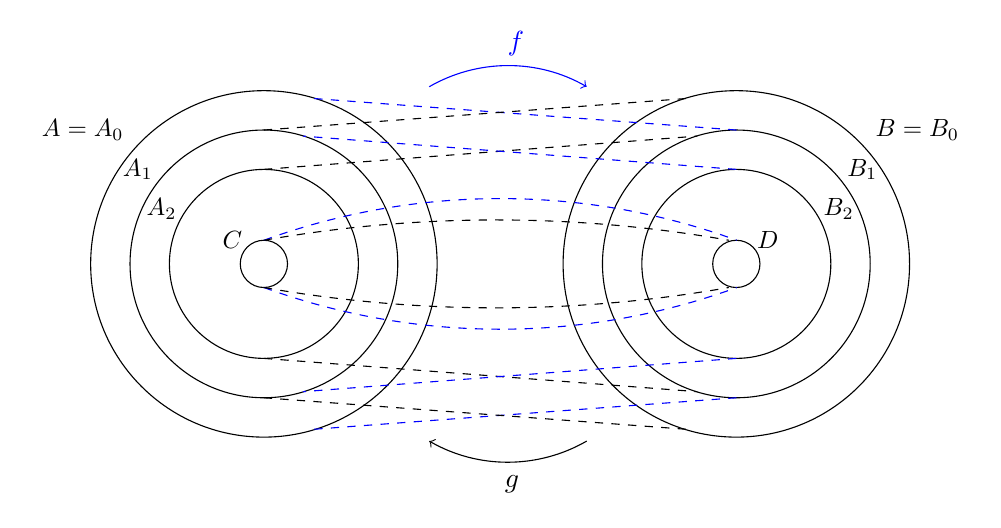
\begin{tikzpicture}
			\clip (-6, -3) rectangle (6, 3);
			
			\draw [] (3, 0) circle[radius=2.2];
			\draw [] (-3, 0) circle[radius=2.2];
			
			\draw [] (3, 0) circle[radius=1.7];
			\draw [] (-3, 0) circle[radius=1.7];
			
			\draw [] (3, 0) circle[radius=1.2];
			\draw [] (-3, 0) circle[radius=1.2];
			
			\draw [] (3, 0) circle[radius=0.3];
			\draw [] (-3, 0) circle[radius=0.3];
			
			\draw[->, blue] (-0.9, 2.25) arc (120:60:2);
			\draw[<-] (-0.9, -2.25) arc (240:300:2);
			
			\draw[dashed, blue] (-3, 0.3) arc (110:70:8.78);
			\draw[dashed] (-3, 0.3) arc (100:80:17);
			\draw[dashed, blue] (-3, -0.3) arc (250:290:8.78);
			\draw[dashed] (-3, -0.3) arc (260:280:17);
			
			\node[blue] at (0.2, 2.8) {$f$};
			\node[] at (0.15, -2.8) {$g$};
			
			\node[] at (3 + 2.3, 1.7) {\scalebox{0.9}{$B = B_0$}};
			\node[] at (3 + 1.6, 1.2) {\scalebox{0.9}{$B_1$}};
			\node[] at (3 + 1.3, 0.7) {\scalebox{0.9}{$B_2$}};
			\node[] at (3 + 0.4, 0.3) {\scalebox{0.9}{$D$}};
			
			\node[] at (-3 - 2.3, 1.7) {\scalebox{0.9}{$A = A_0$}};
			\node[] at (-3 - 1.6, 1.2) {\scalebox{0.9}{$A_1$}};
			\node[] at (-3 - 1.3, 0.7) {\scalebox{0.9}{$A_2$}};
			\node[] at (-3 - 0.4, 0.3) {\scalebox{0.9}{$C$}};
			
			\draw[dashed, blue] (-3 + 0.64, 2.1) -- (3, 1.7);
			\draw[dashed, blue] (-3 + 0.64, -2.1) -- (3, -1.7);
			
			\draw[dashed] (-3, 1.2) -- (3 - 0.495, 1.623);
			\draw[dashed] (-3, -1.2) -- (3 - 0.495, -1.623);
			
			\draw[dashed] (3 - 0.64, 2.1) -- (-3, 1.7);
			\draw[dashed] (3 - 0.64, -2.1) -- (-3, -1.7);
			
			\draw[dashed, blue] (3, 1.2) -- (-3 + 0.495, 1.623);
			\draw[dashed, blue] (3, -1.2) -- (-3 + 0.495, -1.623);
		\end{tikzpicture}
	\end{center}

	Из всего вышесказанного возникают 2 утверждения, которые мы положим в основу биекции $h \colon A \to B$:
	\begin{align*}
	&{f(A_k \bs A_{k + 1}) = B_{k + 1} \bs B_{k + 2}}
	\\
	&{g(B_k \bs B_{k + 1}) = A_{k + 1} \bs A_{k + 2}}
	\end{align*}
	Но этого недостаточно. Ещё могут быть такие элементы, которые не попадут ни в одно кольцо: они принадлежат множествам $C = \bigcap\limits_{i = 0}^\infty A_i$ и $D = \bigcap\limits_{i = 0}^\infty B_i$. Однако при этом заметим, что $f(C) = D$, $g(D) = C$. Если $c \in C$, то $\forall i\ \{c\} \subset A_i$, а из этого следует, что $\forall i\ \{f(c)\} \subset f(A_i)$. Аналогично для $d \in D$. Если же элемент $a \notin C$, то он лежит в каком-то кольце и про этот случай уже всё известно. В итоге получаем следующую биекцию:
	\[
		h(x) = \System{
			&{f(x),\ x \in A_{2k} \bs A_{2k + 1}}
			\\
			&{g^{-1}(x),\ x \in A_{2k + 1} \bs A_{2k + 2}}
			\\
			&{f(x),\ x \in C}
		}
	\]
\end{proof}